\section{Strategy}
\label{Strategy}
We find it interesting to research the design of smarter players, who take into account board characteristics when deciding which marble to place or which sub-board to rotate.
There are two players in the game. Each player has a flag if he is employing a specific strategy or plays randomly. 
To compare two players we use a monte carlo style method: We execute a number of playthroughs until one of the final states is achieved(draw or a player wins).
From these playthroughs we gather the execution time, the number of transitions taken and the result of the game.

\vspace{6pt}

The implemented AI player does two types of moves:
\begin{itemize}
\item Place a marble in a center position
\item Place a marble in the length of another row of own marbles
\end{itemize}

In order to make decisions it first tries to look for a row of 4 marbles and places one marble at either possible end. If this is not available it looks for a row of 3. This patern repeats till the length of the row is 1.

\begin{figure}[!h]
  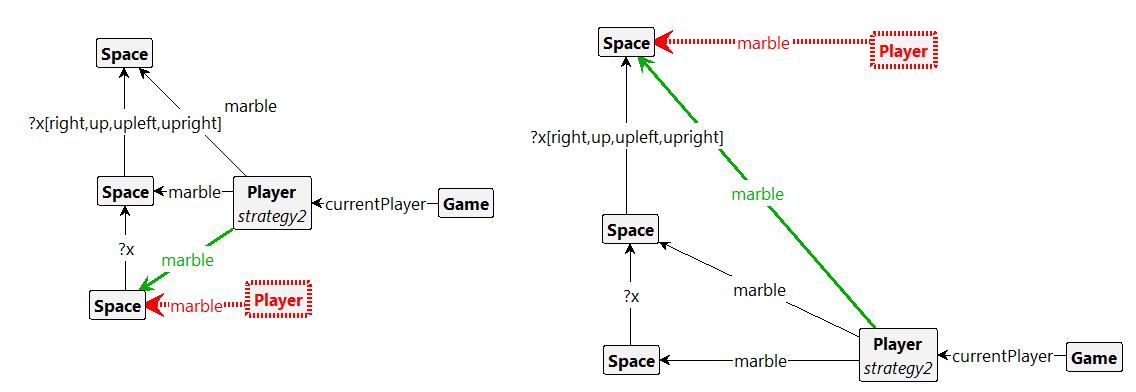
\includegraphics[scale=0.5,clip]{Images/twocombined.png}
  \caption{Types overview}
  \label{fig:twocombined}
\end{figure}
In this section, we describe how smart strategies can be implemented in GROOVE, and we evaluate a smart strategy of our own.

\subsection{Smart block placement}

\subsubsection{Graph}
Tell something about the flag

\subsubsection{Rules}
Tell about the specific rules

\subsubsection{Control Program}
Tell about the control program's function

\subsection{Results}
To be able to draw a conclusion about whether our strategy performs well, we want to formally evaulate its performance.
Because the game is relatively complex, it is impossible to generate the entire state space of the game, and determine the complete win rate of the naive and the smart strategies.
Therefore we have decided to perform a Monte Carlo simulation. A Monte Carlo simulation produces distributions of possible outcome values.

\vspace{6pt}

TODO

To determine the number of iterations needed to meet these requirements, we use the following formula \cite{sim-modeling}:

%n = (zα/2 S / E ) ²
